\documentclass[a4paper, 12pt]{article}
\usepackage[utf8]{inputenc}
\usepackage[T1]{fontenc}
\usepackage[magyar]{babel}
\usepackage{mathtools}
\usepackage{graphicx}
\graphicspath{{../img/}}
\usepackage{hhline}
\usepackage{amsmath}
\usepackage{amssymb}
\usepackage{multicol}
\usepackage{multirow}
\usepackage{anysize}

\marginsize{2.5cm}{2.5cm}{1.8cm}{1.8cm}

\begin{document}

\begin{titlepage}
    \begin{center}
        \vspace*{1cm}
 
        \Huge
        \textbf{Racionális szám osztály\\}
 
        \vspace{0.5cm}
        \Large
	A dokumentum egy C++ nyelvben íródott, racionális szám osztályt megvalósító header fájl készítését bemutató és  tulajdonságait leíró jegyzőkönyv.
 
        \vspace{1.5cm}
 
        \textbf{ Szokody Márk\\}
 
        \vfill

        \large  

        A leírás a\\
       \textbf{ Kutatómunka információs eszközei}\\
        tárgyhoz készült beadandó feladat része.
 
        \vspace{0.8cm}
 
        
\includegraphics[width=0.4\textwidth]{elte.eps}
 
        \Large
        2019.05.18.
 
    \end{center}
\end{titlepage}

\section{Bevezetés}
Jelen jegyzőkönyv a Kutatómunka információs eszközei nevű tárgyhoz készült beadandó feladat. A párhuzamos, Haladó alkalmazott programozás nevű tárgyhoz készített header fájl fejlesztését és működését mutatja be.
Az elkészített feladat GitHubon elérhető, a következő címen:
\begin{center}
https://github.com/szm1000/kutinfo\_bead
\end{center}

\subsection*{A programkódról}
A rational.h fájl egy C++ nyelvhez írt header, mellyel lehetővé válik, hogy a racionális számokat ne lebegőpontosként,
hanem két integer hányadosaként tároljuk. Így kiküszöbölhetővé válnak a kerekítési hibák, azaz a pontosság javul.
A megírás során szempont volt a más osztályokkal való kompatibilitás, így például a racionális osztály példányai eltárolhatók például
egy mátrixban, velük ilyen formában is végezhető művelet. A racionális szám osztály neve Rational.
A feladatkiírásban szerepelt, hogy az osztály legyen használható a Vector2 és Mátrixosztállyal, melyek a tárgy keretei között korábban megírt header fájlok.
A header használatához C++ 17 standard megkövetelése szükséges.

\section{Az elkészítés menete}
\subsection*{Fejlesztési környezet}
A fejlesztést Windows 8.1 Pro 64-bit rendszeren végeztem. A kódot a Microsoft Visual Studio Code programban írtam, a következő bővítményekkel kiegészítve:
\begin{enumerate}
  \item C/C++ for Visual Studio Code 0.23.1 (Microsoft)
  \item C++ Intellisense 0.2.2 (austin)
  \item CMake 0.0.17 (twxs)
  \item CMake Tools 1.1.3 (vector-of-bool)
\end{enumerate}

\begin{figure}[h!]
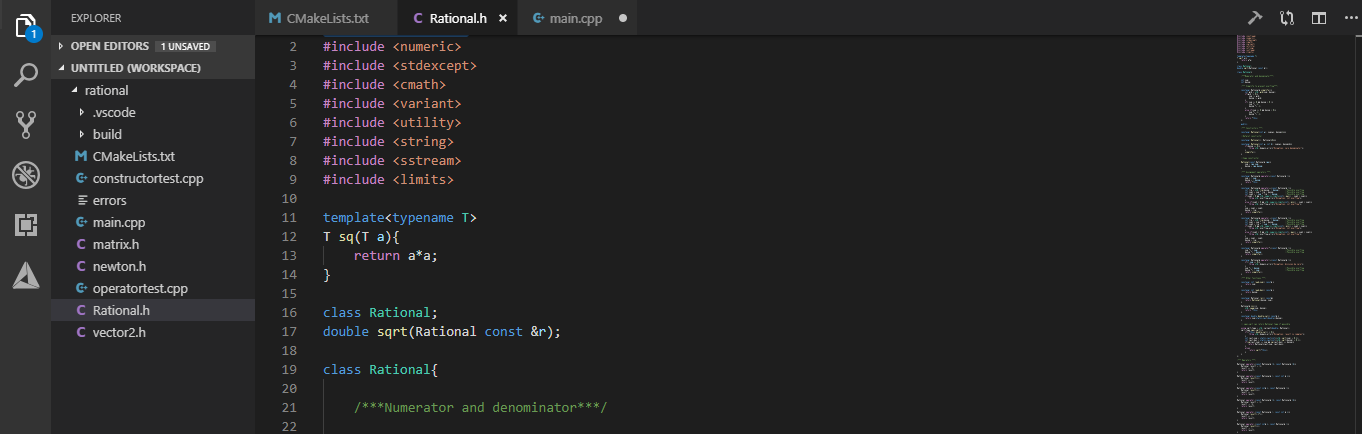
\includegraphics[width=1\textwidth]{vscode.png}
\caption{ Visual Studio Code}
\end{figure}
\newpage
\noindent
A jegyzőkönyvet a MiKTeX implementációval települő TeXworks programban írtam.\\
A program CMake segítségével fordul, így könnyen beállítható volt, hogy a .tex kiterjesztésű fájl is leforduljon a programmal.
\begin{figure}[h!]
\centering
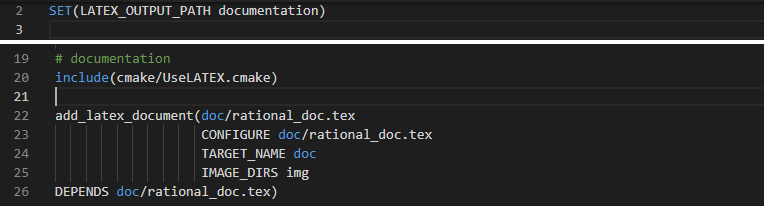
\includegraphics[width=0.8\textwidth]{cmake.png}
\caption{Dokumentáció fordítása CMake-kel}
\end{figure}

\subsection*{Fejlesztési menete}
\indent A programkód megírása során folyamatosan ellenőriztem, a kódrészletek működését.
Először egy kezdetleges verziót készítettem, mely tartalmazta a konstruktorokat, a számláló és nevező kiolvasására szolgáló függvényeket és private elemként a számlálót és nevezőt reprezentáló integereket, valamint az egyszerűsítésre használt simplify() függvényt. 
\\
\indent A második változatban implementáltam az alapvető operátorokat és definiáltam a tárolt szám double formátumú értékét visszaadó függvényt, majd a reciprok, hatvány és gyökvonás függvényekkel bővítettem a kódot.
\\
 Ezek után implementálásra kerültek az összehasonlító és a stream operátorok.
\\
\indent A fejlesztés utolsó szakasza a hibák keresésével és kijavításával telt. Ehhez kikértem a tárgyat tartó oktató véleményét, majd alkalmaztam a javaslatait. Továbbá a feladatnak megfelelően létrehoztam egy Newton iterációval működő, közelítő gyökszámolást elvégző függvényt. A main.cpp tartalmazza a függvények és operátorok tesztjeit, melyek kitérnek az előjelek estleges hibás kezeléséből adódó lehetőségekre is.
Helyes lefutásakor 5 sornyi üzenet jelenik meg, kétszer egy exceptiont és kezelését jelző üzenetpár, valamint egy, a tesztelés végét 
jelző mondat.
\begin{figure}[h!]
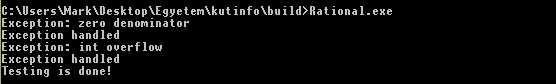
\includegraphics[width=1\textwidth]{succesful.png}
\caption{Sikeres tesztelés esetén látható üzenetek}
\end{figure}

A programot több fordítóval is ellenőriztem, hogy biztosan warning nélkül forduljon. Mivel ez nem igényel nagy kapacitásokat, vagy hosszú futásidőt, internetes fordítókat használtam, melyek már a C++ 17 szabvány szerint működnek.
Ezek a következők:
\begin{itemize}
	\item Coliru: https://coliru.stacked-crooked.com/
	\item OnlineGDB: https://www.onlinegdb.com/online\_c++\_compiler
\end{itemize}

A warning level mindenhol pedantic volt. Ez a CMake fájlban a következőképp állítható be:
\\
\begin{figure}[!h]
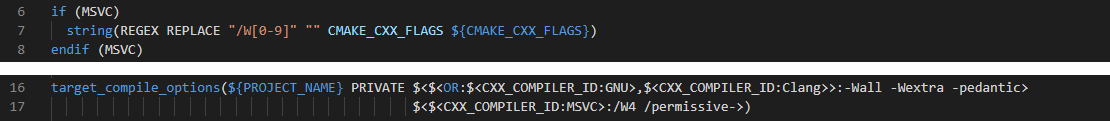
\includegraphics[width=1\textwidth]{cmake3.png}
\caption{Warning level beállítása}
\end{figure}


A fejlesztés nyomonkövethetőségének érdekében a fent leírt mérföldkövek elérése után a kódot feltöltöttem a GitHub repozitóriumba. Ehhez az online felületet használtam.

\begin{figure}[!h]
\centering
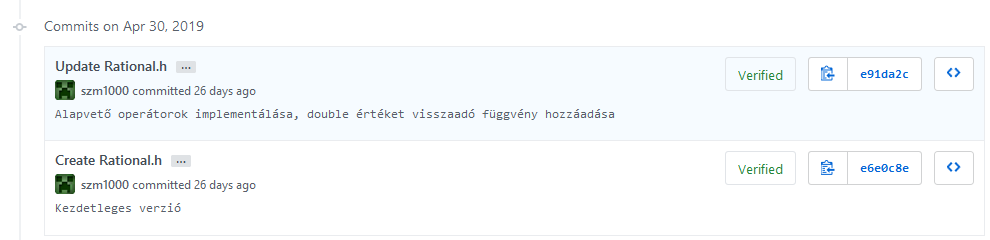
\includegraphics[width=1\textwidth]{github.png}
\caption{GitHub}
\end{figure}

A repozitórium rendelkezik egy readme.md fájllal, ami tartalmazza a fordítás feltételeit, melyek a következők:
\begin{itemize}
    \item CMake 3.8+
    \item ISO C++17 fordító
    \item LaTeX fordító
\end{itemize}

Az első kettő feltétel a CMakeLists.txt fájlban a következőképp néz ki:
\begin{figure}[h!]
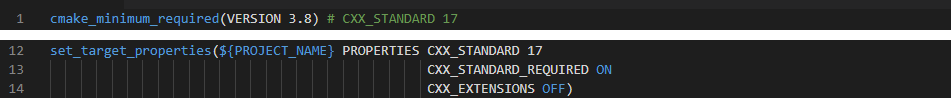
\includegraphics[width=1\textwidth]{cmake2.png}
\caption{C++17 és CMake 3.8 megkövetelése}
\end{figure}

\subsection*{Felmerült problémák}
\indent
Szükségessé vált egy olyan függvény írása, melynek a visszatérési típusa fordítási időben nem ismert, a  lehetséges típusok halmaza viszont igen. Először a boost könyvtár variant függvényét találtam lehetséges megoldásnak, azonban ennek a telepítése során akadályokba ütköztem. Így a további keresés során kiderült, hogy C++ 17-től a Standard Library is rendelkezik azonos funkciójú variant class template-tel. Ez nyilván jobb megoldás, így ez került implementálásra.
\\
\indent
A tesztelést CMake-es unit testekkel szerettem volna elvégezni, azonban a beállítások nem voltak megfelelőek és a határidőig nem találtam megoldást, ezért az egész ellenőrzés a main.cpp-be került.

\section{A header leírása}

\subsection*{Korlátok}
A számláló és a nevező integer típusban van tárolva, így a legkisebb és legnagyobb eltárolható számnak e típus korlátai szabnak határt. 
\newline
Összeadás és kivonás során fellépő esetleges túlcsordulásról a felhasználó kaphat tájékoztatást.
\newline
A tört mindig a legegyszerűbb alakban van tárolva, mivel így csökkenthető a túlcsordulás esélye.
\newline
A negatív előjelet mindig a számláló hordozza.
\newline
Mivel egyes műveletek kivezetnek a racionális számok halmazából, az osztály nem alkalmazható minden esetben a teljes számolásra. 

\subsection*{Az implementált függvények és operátorok}
\subsubsection*{Alapvető műveletek}
Összeadás, kivonás, szorzás, osztás, valamint ezek rövidített változatai(+=, *=, -=, /=). Az összes művelet elvégezhető a Rational osztály példányai között, valamint Rational osztály példánya és integer között. Az összeadás és szorzás mindkét esetben asszociatív.
Két Rational, valamint egy Rational és integer egyenlősége is értelmezve van.
\subsubsection*{simplify()}
Ez a függvény nem public, hanem private. Elvégzi a tört egyszerűsítését a Standard Library gcd függvénye segítségével, illetve rendezi az előjeleket:
\begin{enumerate}
  \item Ha a számláló és a nevező is negatív, mindkettőnek veszi az ellentettjét.
  \item  Ha a számláló pozitív és a nevező negatív, mindkettőnek veszi az ellentettjét.
  \item  Egyéb esetben változatlanul hagyja az előjeleket.
\end{enumerate}
\noindent
 A konstruktorok és az alapvető operátorok mind meghívják ezt a függvényt, így biztosítható, hogy a számok a megfelelő alakban legyenek tárolva.

\subsubsection*{read\_num()}
Visszaadja a számlálót (int) konstans referenciaként.

\subsubsection*{read\_den()}
Visszaadja a nevezőt (int) konstans referenciaként.

\subsubsection*{rec()}
Visszaadja a tört reciprokát (Rational) konstans referenciaként.

\subsubsection*{inv()}
Felcseréli a számlálót és nevezőt a Standard Library swap függvénye segítségével. 

\subsubsection*{double\_val()}
Visszaadja a tört értékét double típussal, konstans referenciaként.

\subsubsection*{spec\_sqrt()}
Visszaadja a tört gyökét, ha lehetséges Rational alakban, ha nem akkor double típussal, a Standard Library-ban lévő variant (C++17)  segítségével. Ha a tört negatív, \\domain\_error típusú standard hibát jelent.

\subsubsection*{Összehasonlító operátorok}
Globális definíció az == és a < operátorokra. A további összehasonlítást végző operátorhoz az Standard Library rel\_ops névterének használatával juthatunk hozzá.

\subsubsection*{sqrt(Rational const\&)}
Globálisan definiált függvény. Visszaadja a tört gyökét double típussal. Ha a tört negatív, domain\_error típusú standard hibát jelent.

\subsubsection*{newton\_sqrt(double, double, int, double)}
Globálisan definiált függvény. Visszaadja a tört gyökének közelítő értékét double típussal. Ha a tört negatív, domain\_error típusú standard hibát jelent.

\subsubsection*{pow(Rational const\& , int const\&)}
Globálisan definiált függvény. Visszaadja a tört integer paraméterrel megadott hatványát Rational típussal. A Standard Library pow() függvényét használja. Ha a számláló vagy nevező túlcsordulna, overflow\_error típusú standard hibát jelent.

\subsubsection*{pow(Rational const\& , double const\&)}
Globálisan definiált függvény. Visszaadja a tört double paraméterrel megadott hatványát double típussal. A Standard Library pow() függvényét használja.

\subsubsection*{abs(Rational const\&)}
Globálisan definiált függvény. Visszaadja a tört abszolút értékét Rational típussal, a Standard Library abs() függvényének segítségével.

\subsubsection*{Stream operátorok}
A << operátor kiírja a streambe a Rational típust "számláló/nevező " formátumban. A >> operátorral lehetővé válik Rational típus beolvasása megfelelő formátum esetén.

\subsection*{Exceptionok}
\begin{enumerate}
  \item Inicializálásnál, ha a nevező nulla: \\std::domain\_error\{"Exception: zero denominator"\}
  \item Összeadásnál és kivonásnál túlcsordulás esetén:\\ std::overflow\_error\{"Exception: int overflow"\}
  \item Nullával való osztásnál: \\std::domain\_error\{"Exception: division by zero"\}
  \item Gyökvonásnál, ha a szám negatív: \\std::domain\_error\{"Exception: result is complex"\}
  \item Hatványozásnál túlcsordulás esetén: \\std::overflow\_error\{"Exception: int overflow"\}
\end{enumerate}


\section{Kiegésztés}
A C++20-tól elérhető a Standard Library-ben a concepts, melynek segítségével általánosítani lehet a típust, ezáltal választani lehetne int vagy long típusok között.


\end{document}
